
\documentclass{article}
\usepackage{amsmath,amssymb}
\usepackage[inline]{enumitem}
\usepackage{blindtext}
\usepackage{booktabs}
\usepackage{graphicx}
\usepackage{xcolor}
\usepackage[vmargin = 1.5in, top = 1in, bottom = 1.2in, letterpaper]{geometry}
\usepackage{listings}
\usepackage{courier}
\usepackage{multicol}
\usepackage{multirow}
\usepackage{bm}
\lstset{
basicstyle = \small\tt,
keywordstyle = \tt\color{blue},
commentstyle = \it\color[cmyk]{1,0,1,0},
stringstyle = \tt\color[RGB]{128,0,0},
%frame = single,
backgroundcolor = \color[RGB]{245,245,244},
breaklines,
extendedchars = false,
xleftmargin = 2em,
xrightmargin = 2em,
aboveskip = 1em,
tabsize = 4,
showspaces = false
}
\begin{document}
\setcounter{MaxMatrixCols}{20}

% \newfontfamily\courier{Courier New}


\title{STAT 510 Homework 9}
\author{Yifan Zhu}
\maketitle

\begin{enumerate}[leftmargin = 0 em, label = \arabic*., font = \bfseries]
	\item
	\begin{enumerate}
		\item \ 

		\begin{tabular}{l|rrr}
		\toprule
			& \multicolumn{3}{c}{geno}\\
			fert & 1 & 2 & 3\\
			\hline
			0 & 125 & 140 & 115\\
			50 & 141.25 & 156.25 & 141.25\\
			100 & 150 & 165 & 160 \\
			150 & 151.25 & 166.25 & 171.25\\
			\bottomrule
		\end{tabular}

		\item 
		Not true.
		\item 
		Not true.
		\item 
		Not true.
		\item 
		Geno Type 1:
		\[ E(y) = 125 + 0.4 f -0.0015 f^2\]
		Geno Type 2:
		\[ E(y) = 140 + 0.4 f - 0.0015 f^2\]
		Geno Type 3:
		\[ E(y) = 115 + 0.6 f - 0.0015 f^2\]

		\begin{center}
			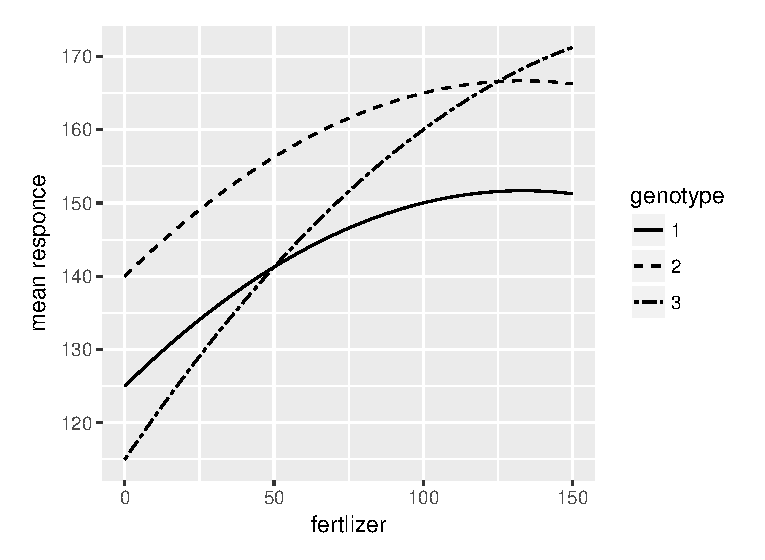
\includegraphics[width = 0.7\textwidth]{Rplot.eps}
		\end{center}

		\item 
		$\bar{y}_{11 \cdot} - \bar{y}_{12 \cdot} = -13.75,\, SE = \sqrt{\frac{\hat{\sigma}_{e}^2}{2}} = \frac{6.30128}{\sqrt{2}}$. 

		$CI = (\bar{y}_{11 \cdot} - \bar{y}_{12 \cdot} - SE \cdot t_{27, 0.975} ,\bar{y}_{11 \cdot} - \bar{y}_{12 \cdot} + SE \cdot t_{27, 0.975} ) = ( -22.8923, -4.607704)$. 
		\item 
		$\mu_{11} - \mu_{12} = -15 \in CI = (-22.8923, -4.607704)$.

		\item 
		$\bar{y}_{11} - \bar{y}_{21} = -22.5,\, SE = \frac{\sqrt{\hat{\sigma}_e^2 + \hat{\sigma}_w^2}}{\sqrt{2}} = \sqrt{\frac{39.70613 + 67.2981}{2}} =  7.314514,\, df = \frac{\left( \frac{1}{4} MS_{Block \times Geno} + \frac{3}{4} MS_{Error} \right)^2 }{\frac{1}{16} \frac{MS_{Block \times Geno}^2}{6} + \frac{9}{16} \frac{MS_{Error}^2}{27}} = 8.88$. 

		$CI = (\bar{y}_{11 \cdot} - \bar{y}_{21 \cdot} - SE \cdot t_{27, 0.975} ,\bar{y}_{11 \cdot} - \bar{y}_{12 \cdot} + SE \cdot t_{8.88, 0.975} ) = ( -39.08073, -5.919272)$.

		\item 
		$\mu_{11} - \mu_{21} = -16.25 \in CI = ( -39.08073, -5.919272)$.

		\item 
		$SE = \frac{\hat{\sigma}_b^2}{4}+\frac{\hat{\sigma}_w^2}{12} + \frac{\hat{\sigma}_e^2}{48} = \frac{MS_{Block}}{48},\, df = 4-1 = 3$. 
	\end{enumerate}
	

	\item 
	\begin{enumerate}
		\item 
		\[\frac{MS_{\mathrm{WL}}}{MS_{\mathrm{GH:WL}}} = \frac{160.9}{19.4} = 8.29\]

		\item 
		\[\frac{MS_{\mathrm{GENO}}}{MS_{\mathrm{Error}}} = \frac{MS_{\mathrm{GENO}}}{\frac{SS_{\mathrm{GH:GENO}} + SS_{\mathrm{GENO : WL : GENO}}} {3+6}} = \frac{2.5}{\frac{11.7 + 14.5}{3+6}} = \frac{2.5}{2.92} = 0.856\]

		\item
		\[\frac{MS_{\mathrm{WL:GENO}}}{MS_{\mathrm{Error}}} = \frac{37.5}{2.92} = 12.84\] 
	\end{enumerate}

	\item 
	\begin{enumerate}
		\item 
		$avg_{ik} = a_{ik} = \bar{\mu}_{i \cdot} + p_k + \bar{e}_{i \cdot k}$, then $\bar{a}_{1 \cdot} = \bar{\mu}_{1 \cdot} + \frac{1}{6} \sum_{k=1}^6 p_k + \frac{1}{6} \sum_{k=1}^6 \bar{e}_{1 \cdot k},\, \bar{a}_{2 \cdot} = \bar{\mu}_{2 \cdot} + \frac{1}{12} \sum_{k=7}^{18} p_k + \frac{1}{12} \sum_{k=7}^{18} \bar{e}_{2 \cdot k}$. Hence we have 
		\[Var\left(\bar{a}_{1 \cdot}\right) = \frac{1}{6} \sigma_p^2 + \frac{1}{6} \frac{1}{2} \sigma_e^2 = \frac{\sigma_p^2}{6} + \frac{\sigma_e^2}{12},\, Var(\bar{a}_{2 \cdot}) = \frac{1}{12} \sigma_p^2 + \frac{1}{12} \frac{1}{2} \sigma_e^2 = \frac{1}{2} Var(\bar{a}_{1 \cdot})\]
		Note that $\bar{a}_{1 \cdot} - \bar{a}_{2 \cdot} = \bar{\mu}_{1 \cdot} - \bar{\mu}_{2 \cdot} + \frac{1}{6} \sum_{k=1}^6 \left(  p_k + \bar{e}_{1 \cdot k}\right) + \frac{1}{12}  \sum_{k=7}^{18}\left( p_k + \bar{e}_{2 \cdot k} \right)$, and $Var(\bar{a}_{1 \cdot} - \bar{a}_{2 \cdot}) = \frac{1}{6} \sigma_p^2 + \frac{1}{12} \sigma_p^2 + \frac{1}{12} \sigma_e^2 + \frac{1}{24} \sigma_e^2 = \frac{1}{4} \sigma_p^2 + \frac{1}{8} \sigma_e^2$. Thus test statistic is 
		\[T = \frac{84.892 - 80.454}{\sqrt{2.169^2 + 1.534^2}} = 1.6705\]

		\item 
		$diff_{ik} = d_{ik} = \mu_{i1} - \mu_{i2} + e_{i1k} - e_{i2k}$, then $Var(\bar{d}_{1 \cdot}) = Var\left(\mu_{11} - \mu_{12} + \frac{1}{6} \sum_{k=1}^6 (e_{11k} - e_{12k})\right) = \frac{1}{6} 2 \sigma_e^2 = \frac{1}{3} \sigma_{e}^2, \,Var(\bar{d}_{2 \cdot}) = Var\left(\mu_{21} - \mu_{22} + \frac{1}{12} \sum_{k=7}^{18} (e_{21k} - e_{22k})\right) = \frac{1}{12} 2 \sigma_e^2 = \frac{1}{6} \sigma_{e}^2 = \frac{1}{2} Var(\bar{d}_{1 \cdot}).$ 

		Note that $\frac{1}{2} (\bar{d}_{1 \cdot} + \bar{d}_{2 \cdot}) = \bar{\mu}_{ \cdot 1} - \bar{\mu}_{ \cdot 2} + \frac{1}{12} \sum_{k=1}^6 (e_{11k} - e_{12k}) + \frac{1}{24} \sum_{k=7}^{18}(e_{21k} - e_{22k}) $ and $Var(\frac{1}{2}(\bar{d}_{1 \cdot} + \bar{d}_{2 \cdot})) = \frac{1}{8} \sigma_e^2$. Hence the test statistic
		\[T = \frac{ \frac{1}{2} (8.25 + 1.492)}{\sqrt{\frac{1}{4} (2.439^2 + 1.724^2)}} = 3.262\]

		\item 
		$\bar{y}_{11 \cdot} - \bar{y}_{12 \cdot} - \bar{y}_{21 \cdot} + \bar{y}_{22 \cdot} = \mu_{11} - \mu_{12} - \mu_{21} + \mu_{22} + \frac{1}{6} \sum_{k=1}^6 p_k + \frac{1}{6}\sum_{k=1}^6 e_{11k} - \frac{1}{6} \sum_{k=1}^6 p_k - \frac{1}{6} \sum_{k=1}^6 e_{12k} - \frac{1}{12} \sum_{k=7}^{18} p_k - \frac{1}{12} e_{21k} + \frac{1}{12} \sum_{k=7}^18 p_k + \frac{1}{12} \sum_{k=7}^{18} e_{22k} = \mu_{11} - \mu_{12} - \mu_{21} + \mu_{22} + \bar{e}_{11 \cdot} - \bar{e}_{12 \cdot} - \bar{e}_{21 \cdot} + \bar{e}_{22 \cdot}$. And $Var(\bar{y}_{11 \cdot} - \bar{y}_{12 \cdot} - \bar{y}_{21 \cdot} + \bar{y}_{22 \cdot}) = \frac{1}{6} \sigma_e^2 + \frac{1}{6} \sigma_e^2 + \frac{1}{12} \sigma_{e}^2 + \frac{1}{12} \sigma_e^2 = \frac{1}{2} \sigma_e^2$. We also know that $(\bar{y}_{11 \cdot} - \bar{y}_{12 \cdot} - \bar{y}_{21 \cdot} + \bar{y}_{22 \cdot})^2/(1/6 + 1/6 + 1/12 + 1/12) = MS_{\mathrm{geno:infection}} \Rightarrow \bar{y}_{11 \cdot} - \bar{y}_{12 \cdot} - \bar{y}_{21 \cdot} + \bar{y}_{22 \cdot} = \sqrt{91.35/2} = 6.758$. Then test statistic
		\[T = \frac{6.758}{\sqrt{2.439^2 + 1.724^2}} = 2.263\]

		\item 
		$\hat{\sigma}_e^2 = {(2.439^2 + 1.724^2)\times 2} = 17.84$
		\item 
		$\hat{\sigma}_p^2 = (2.169^2 + 1.534^2) \times 4 - 17.84/2 = 19.31$.
	\end{enumerate}
	
	     
\end{enumerate}
	      

\end{document}